\chapter{Paraxial Wave Multipath Propagation Model}
\label{analytical_propagation}

This section derives the solution for the multiple ray model in the paraxial assumption and demonstrates that it is asymptotically equivalent to the 2 ray model. The 2-Ray multipath model over a flat earth is given in Figure \ref{mp_fig:1}. In this figure, $P_1$ and $P_2$ are the two points we are interested in propagating between and $P_2'$ is the mirror image of $P_2$. $L_1$ is then the direct path and $L_{so}$ represents the shortest orbit reflection from the sea surface. The altitudes of the two points from the mean sea surface are $h_1$ and $h_2$, the total downrange distance is $L$, and the distance to the reflection point is $x_m$.

\begin{figure}[H]
  \begin{center}
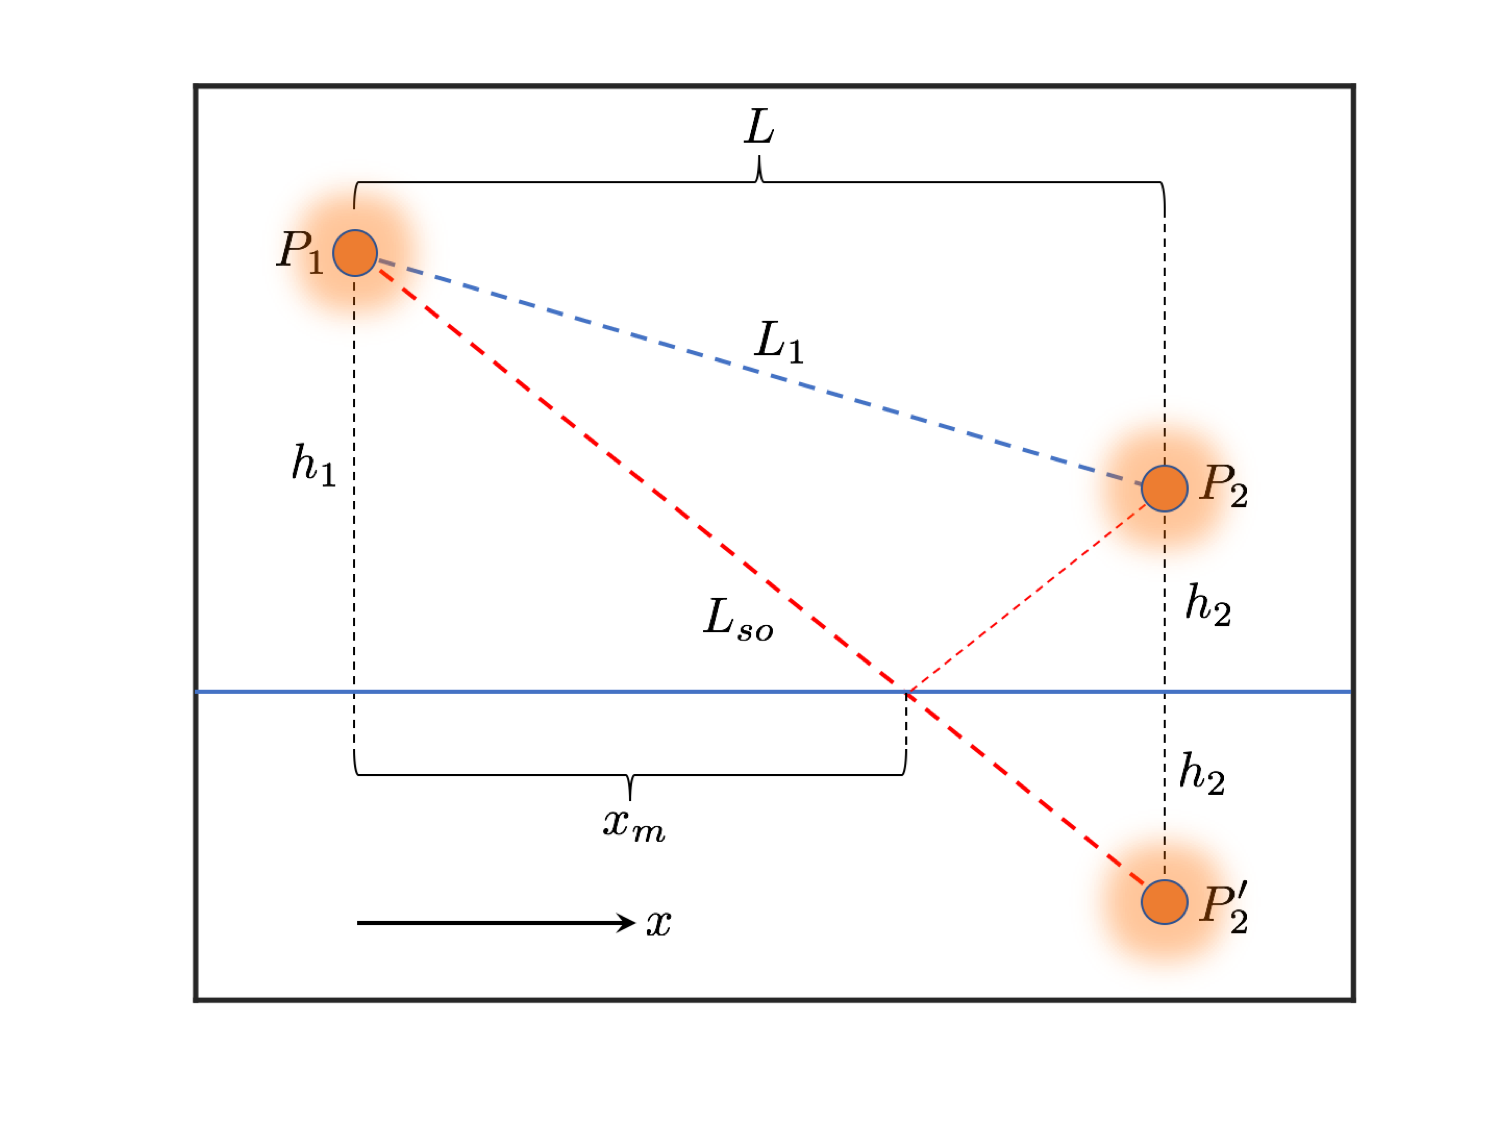
\includegraphics[width=5in]{../media/analysis/multipath_2_ray.png}
  \end{center}
  \renewcommand{\baselinestretch}{1} \small\normalsize
  \begin{quote}
    \caption[2 Ray Multipath Geometry]{ 2 Ray Multipath Geometry\label{mp_fig:1}}
  \end{quote}
\end{figure}
\renewcommand{\baselinestretch}{2} \small\normalsize

To capture the effects of propagating over a spherical earth, the altitude $h_2$ can be modified with a correction factor \cite{blake_radar} dependent on the effective radius of the earth, $r_e = (4/3) 6,371,000$ m.
\begin{equation}
h_2' = h_2 - \frac{L^2}{2r_e}
\label{mp_eq:0}
\end{equation}

The path lengths are given by geometry and simplified through a binomial expansion.
\begin{equation}
\begin{aligned}
L_1 & = \sqrt{L^2 + (h_1-h_2)^2}  \approx L + \frac{(h_1 - h_2)^2}{2L}\\
L_{so} & = \sqrt{L^2 + (h_1+h_2)^2}  \approx L + \frac{(h_1 + h_2)^2}{2L}\\
\end{aligned}
\label{mp_eq:1}
\end{equation}
\renewcommand{\baselinestretch}{2} \small\normalsize

From Huygen's principle, the propagation factor for the 2-ray model is the sum of plane waves traveling along the paths $L_1$ and $L_{so}$. Here $\Gamma_1$ is the reflection coefficient from the sea surface, $\Gamma_1 = \Gamma(x_m)$.
\begin{equation}
\boxed{F_p = e^{jkL_1} + \Gamma_1e^{jkL_{so}}}
\label{mp_eq:1b}
\end{equation}

\section{Geometry}
To include multiple rays, we must consider the region over which the electromagnetic wave reflects from the surface, $\tilde{x}$, as shown in Figure \ref{mp_fig:2}, which extends Figure \ref{mp_fig:1}. Here, $L_2$ and $L_3$ are the path lengths for the various reflected rays and $s(x)$ is the altitude of the sea surface at $x$. 

\begin{figure}[H]
  \begin{center}
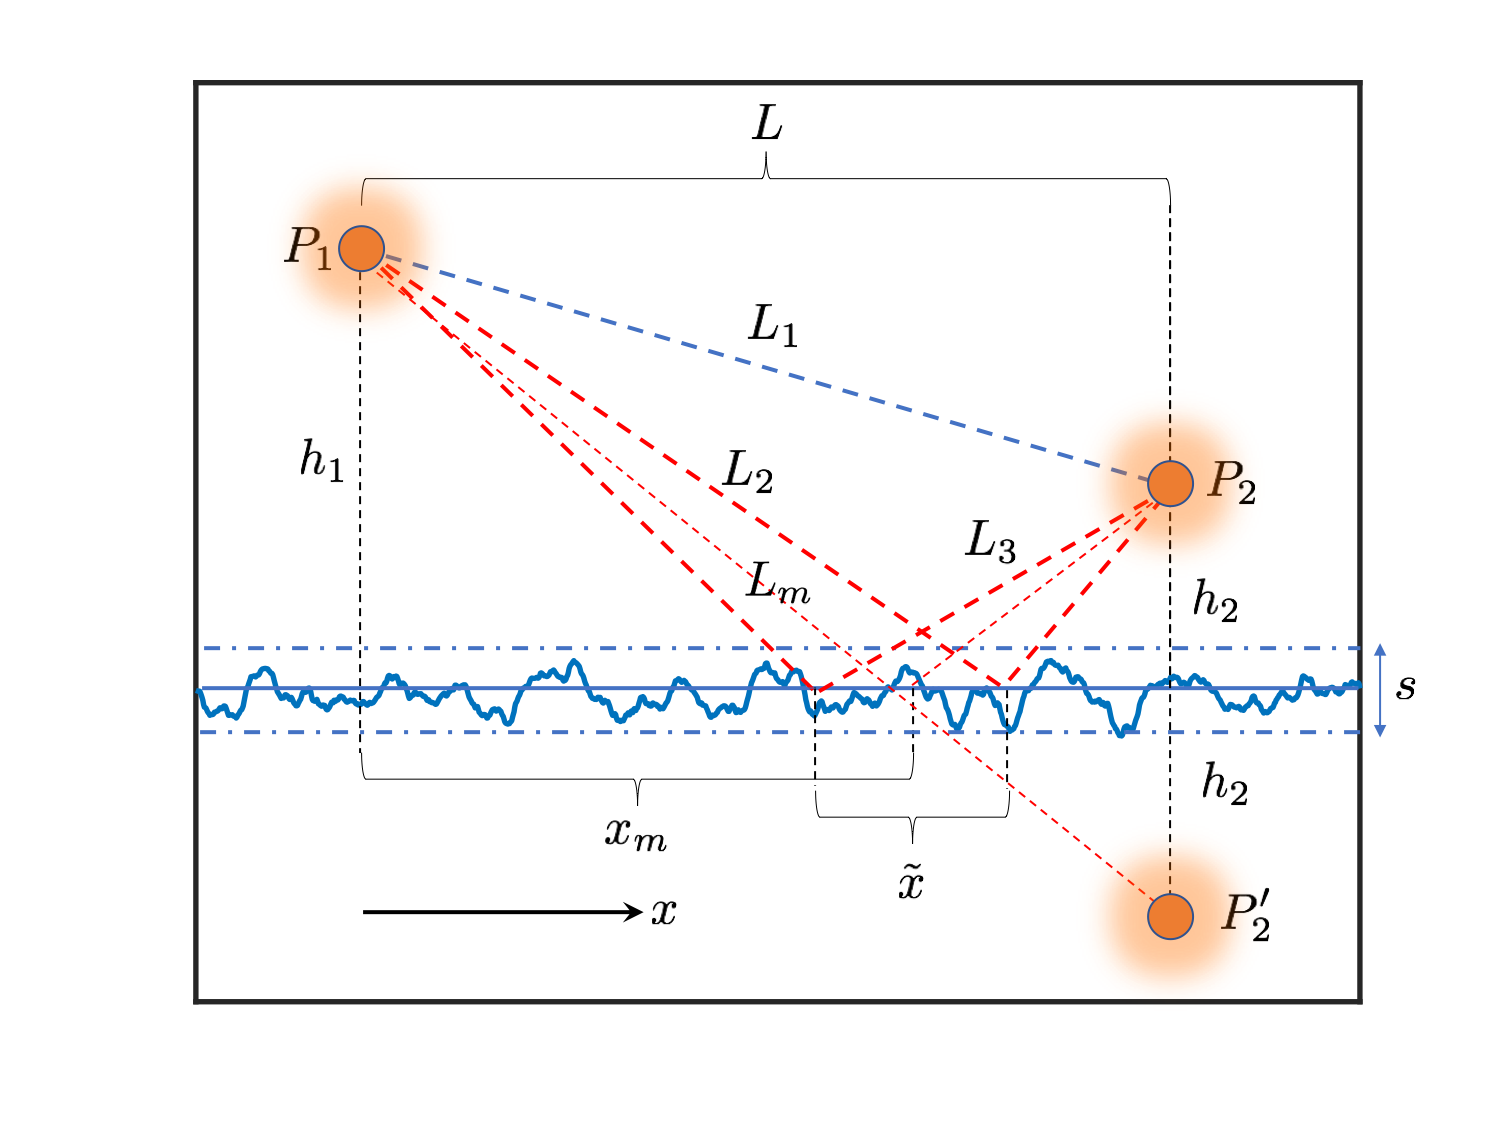
\includegraphics[width=5in]{../media/analysis/multipath_layout.png}
  \end{center}
  \renewcommand{\baselinestretch}{1} \small\normalsize
  \begin{quote}
    \caption[Multipath Geometry for Multiple Ray Analysis]{Multipath Geometry for Multiple Ray Analysis\label{mp_fig:2}}
  \end{quote}
\end{figure}
\renewcommand{\baselinestretch}{2} \small\normalsize

The path lengths  $L_2$ and $L_3$ for the reflected ray can be defined through similar triangles around $x$ and can again be simplified through a binomial expansion. At high altitudes or small sea states, $2h_1s(x) >> s^2(x)$ and we can neglect the $s^2(x)$ term.
\begin{equation}
\begin{aligned}
L_2 &= \sqrt{x^2 + \left( h_1 - s(x)\right)^2}  \approx x + \frac{(h_1-s(x))^2}{2x}\\
L_3 & = \sqrt{\left(L - x\right)^2 + \left( h_2 - s(x)\right)^2}  \approx L-x + \frac{(h_2 - s(x))^2}{2\left(L-x\right)}\\
\end{aligned}
\label{mp_eq:12}
\end{equation}
\renewcommand{\baselinestretch}{2} \small\normalsize

\section{Path Approximations and Expansions}
The path length for a given reflected ray, $L_r$ is given by
\begin{equation}
\begin{aligned}
L_r &= L_2 + L_3 \\
& = x + \frac{h_1^2-2h_1s(x)}{2x} +  L-x + \frac{h_2^2 - 2h_2s(x)}{2\left(L-x\right)} \\
& = L + \frac{1}{2}\left[\frac{h_1^2}{x} + \frac{h_2^2}{L-x} \right] - s(x)\left[ \frac{h_1}{x} + \frac{h_2}{L-x}\right] \\
&= L + L_0 - L_s
\end{aligned}
\label{mp_eq:13}
\end{equation}
\renewcommand{\baselinestretch}{2} \small\normalsize

Here $L_0$ represents the deterministic component due to reflection from the surface and $L_s$ represents the random component due to reflection from the surface. The reflection point from the 2-ray model, $x_m$, should be a saddle point and provide the dominant contribution. We can therefore perform a Taylor expansion of $L_0$ about $x_m$.

\begin{equation}
L_0 \approx L_0(x_m) + \frac{1}{2}\frac{d^2L_0}{dx^2}\bigg|_{x_m}(x-x_m)^2
\label{mp_eq:14}
\end{equation}

\begin{equation}
\frac{dL_0}{dx} = \frac{1}{2}\left[\frac{-h_1^2}{x^2} + \frac{h_2^2}{(L-x)^2} \right]
\label{mp_eq:15}
\end{equation}

\begin{equation}
\frac{d^2L_0}{dx^2} = \frac{h_1^2}{x^3} + \frac{h_2^2}{(L-x)^3} 
\label{mp_eq:16}
\end{equation}

Since $\frac{dL_0}{dx}\big|_{x_m} = 0$, we can solve for $x_m$
\begin{equation}
\begin{gathered}
\frac{-h_1^2}{x_m^2} + \frac{h_2^2}{(L-x_m)^2} = 0\\
\frac{-h_1}{x_m} + \frac{h_2}{L-x_m} = 0\\
\frac{h_1}{x_m} = \frac{h_2}{L-x_m}\\
h_1(L-x_m) = h_2x_m\\
x_m = \frac{h_1L}{h_1+h_2}
\end{gathered}
\label{mp_eq:17}
\end{equation}

This gives the following for the lowest Taylor series terms:
\begin{equation}
\begin{aligned}
L_0(x_m) &= \frac{(h_1+h_2)^2}{2L} \\
L_0''\frac{d^2L_0}{dx^2}\bigg|_{x_m}  &= \frac{(h_1+h_2)^4}{h_1h_2L^3} \\
L_s(x_m) &= \frac{2s(x)(h_1 + h_2)}{L}\\
\end{aligned}
\label{mp_eq:17a}
\end{equation}

The expansion of $L_0$ is then
\begin{equation}
L_0 \approx \frac{(h_1+h_2)^2}{2L} + \frac{(h_1+h_2)^4}{2h_1h_2L^3}(x-x_m)^2
\label{mp_eq:18}
\end{equation}

\section{Solution Through Green's Functions}
The Green's function for the paraxial wave equation is derived in Section \ref{gf_sec:paraxial} as
\begin{equation}
G\left(x,x',z,z' \right)= \sqrt{\frac{j}{8\pi k_o|x-x'|}}\exp\left[-jk_o\left(|x -x'| + \frac{|z-z'|^2}{2|x-x'|}\right) \right]
\label{mp_eq:11aa}
\end{equation}
\renewcommand{\baselinestretch}{2} \small\normalsize
Where the source is located at $(x',z')$ and the observation point is located at $(x,z)$.

\subsection{Direct Path}
The solution to the scalar wave equation at $P_2$ for the direct path can be found by using the Green's function from equation \ref{mp_eq:11aa} with a delta function at $P_1$ ($x' = 0, z' = h_1$) representing a point source.

\begin{equation}
\begin{gathered}
U_1(P_2) = \int_{-\infty}^{\infty} \int_{-\infty}^{\infty}dx' dz' G\left(x,x',z,z' \right) f(x',z') \\
U_1(P_2) = \int_{-\infty}^{\infty} \int_{-\infty}^{\infty}dx' dz' G\left(x,x',z,z' \right)\delta(x') \delta(z'- (h_1-s)) \\
U_1(P_2) = \int_{-\infty}^{\infty} \int_{-\infty}^{\infty}dx' dz' \sqrt{\frac{j}{8\pi k_o|x-x'|}}\exp\left[-jk_o\left(|x -x'| + \frac{|z-z'|^2}{2|x-x'|}\right) \right] \\
\times \delta(x') \delta(z'- (h_1-s)) \\
U_1(P_2) = \frac{1}{2jk_o}\sqrt{\frac{k_o}{2\pi jx}}\exp\left[-jk_o\left(x + \frac{(z-(h_1-s))^2}{2(x)}\right) \right]\\
\end{gathered}
\label{mp_eq:11ab}
\end{equation}
\renewcommand{\baselinestretch}{2} \small\normalsize

At $P_2$, $x = L$ and $z = h_2-s$, so the direct path can be written as
\begin{equation}
\begin{gathered}
U_1(P_2) = \frac{1}{2jk_o}\sqrt{\frac{k_o}{2\pi jL}}\exp\left[-jk_o\left(L + \frac{((h_2-s)-(h_1-s))^2}{2L}\right) \right]\\
=\frac{1}{2jk_o} \sqrt{\frac{k_o}{2\pi jL}}\exp\left[-jk_oL_1 \right]\\
\end{gathered}
\label{mp_eq:11ac}
\end{equation}
\renewcommand{\baselinestretch}{2} \small\normalsize

\subsection{Rayleigh-Sommerfeld Diffraction Integral}
Following Huygen's principle, we can use every point on the sea surface as a source for the reflected wave. We will follow \cite{goodman_fourier} and treat diffraction from the sea surface similarly to diffraction from a planar screen. 

The scalar solution from the Green's function method is derived in Section \ref{gf_sec:method} as
\begin{equation}
U = \oint\limits_{S}\left[G\frac{\partial U}{\partial n}dS - U\frac{\partial G}{\partial n} \right] -\int\limits_{V}d^3r' Gf
\label{mp_eq:11aaa}
\end{equation}
\renewcommand{\baselinestretch}{2} \small\normalsize

We will focus here on the homogeneous solution, $f=0$, and let the surface normal direction, $\hat{n}$, be along $z$. In order to ensure the integral over the surface vanishes at far distances, we need to apply the Sommerfeld radiation condition on the disturbance $U$
\begin{equation}
 \lim_{x\to\infty} x\left(\frac{\partial U}{\partial z} -jkzU \right) = 0.
\label{mp_eq:11aaaa}
\end{equation}
\renewcommand{\baselinestretch}{2} \small\normalsize

In order the simplify the surface integral in Equation \ref{mp_eq:11aaa}, we can choose an alternative Green's function that is generated by a pair of mirrored point sources as shown in Figure \ref{mp_fig:2a}. This configuration will ensure that the Green's function vanishes on the surface provided that the assumption of small altitude deviations along the surface holds.

\begin{figure}[H]
  \begin{center}
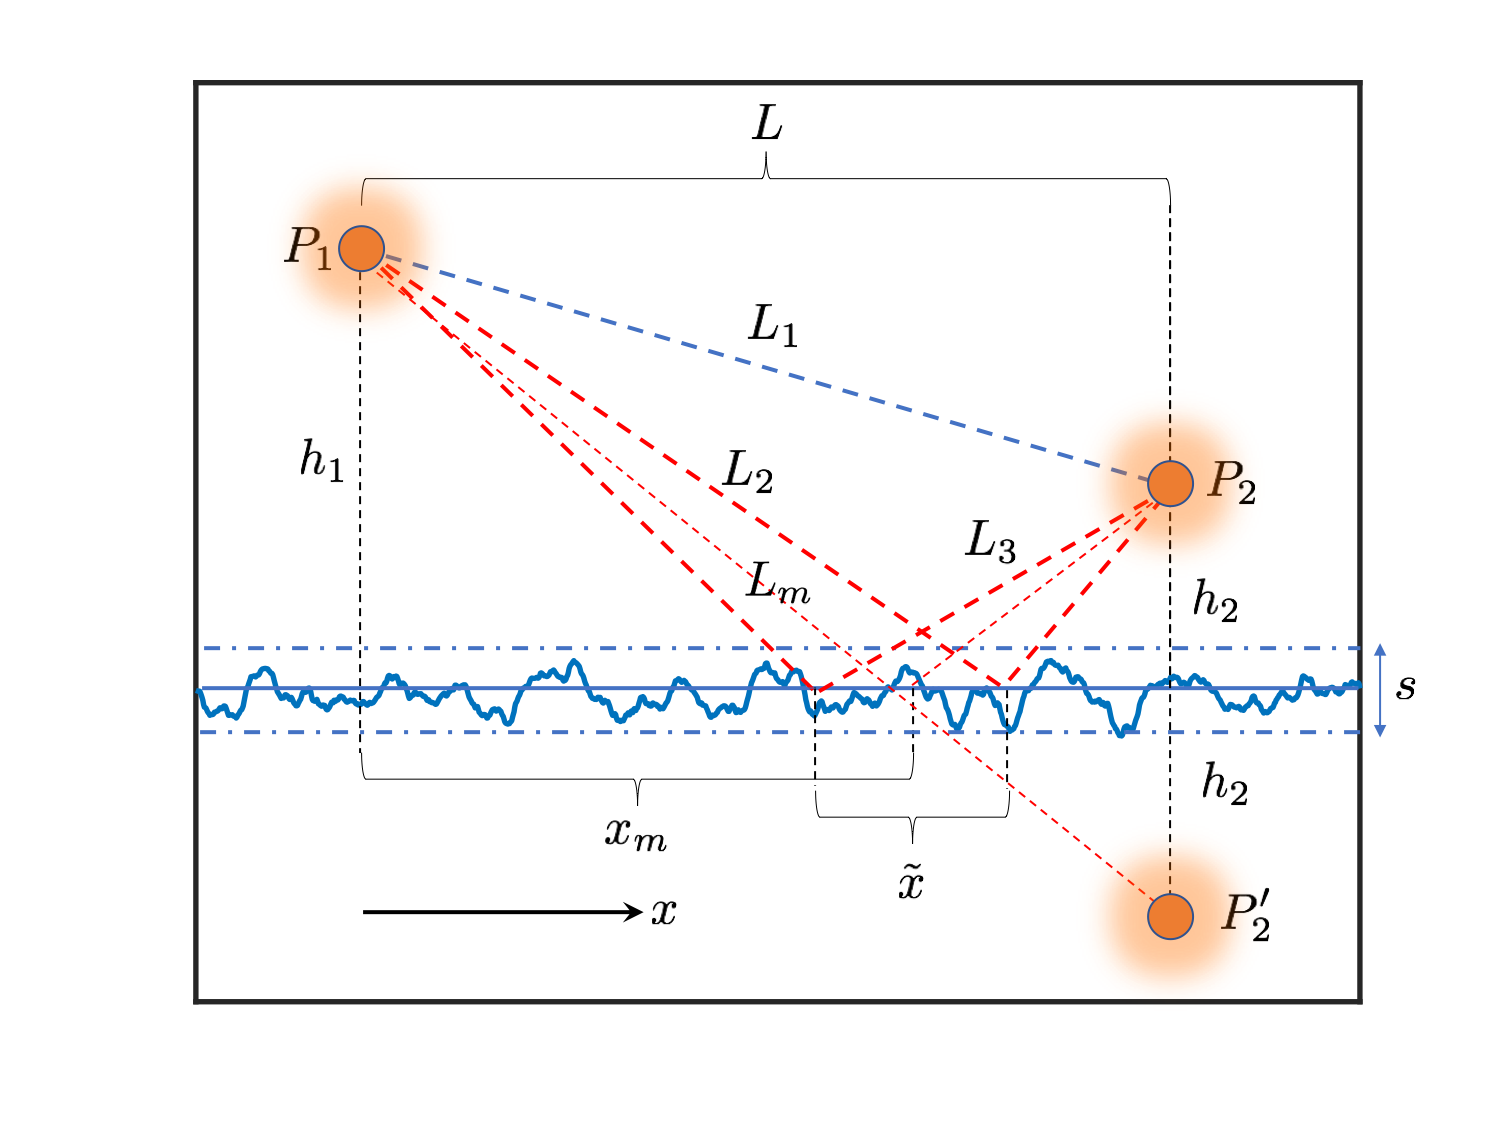
\includegraphics[width=5in]{../media/analysis/multipath_layout.png}
  \end{center}
  \renewcommand{\baselinestretch}{1} \small\normalsize
  \begin{quote}
    \caption[Rayleigh-Sommerfeld Green's Function Geometry]{Rayleigh-Sommerfeld Green's Function Geometry\label{mp_fig:2a}}
  \end{quote}
\end{figure}
\renewcommand{\baselinestretch}{2} \small\normalsize

This Greens function, $G\_$, is then given as
\begin{equation}
G\_= \sqrt{\frac{j}{8\pi k_ox}}\exp\left[-jk_o\left(x + \frac{z^2}{2x}\right) \right] - \sqrt{\frac{j}{8\pi k_ox_1}}\exp\left[-jk_o\left(x_1 + \frac{z_1^2}{2x_1}\right) \right]
\label{mp_eq:11aab}
\end{equation}
\renewcommand{\baselinestretch}{2} \small\normalsize

The normal derivative $\partial G\_/\partial n$, is then given as
\begin{equation}
\begin{aligned}
\frac{\partial G\_}{\partial n}&-\frac{jk_oz}{x}\sqrt{\frac{j}{8\pi k_ox}}\exp\left[-jk_o\left(x + \frac{z^2}{2x}\right) \right] \\
&-\frac{jk_oz_1}{x_1}\sqrt{\frac{j}{8\pi k_ox_1}}\exp\left[-jk_o\left(x_1 + \frac{z_1^2}{2x_1}\right) \right]
\end{aligned}
\label{mp_eq:11aac}
\end{equation}
\renewcommand{\baselinestretch}{2} \small\normalsize

On the surface, $x_1 = x$ and $z_1 = -z$ so that
\begin{equation}
\begin{gathered}
\frac{\partial G\_}{\partial n} = -2\frac{\partial G}{\partial n} \\
\frac{\partial G\_}{\partial n} = -2jk_o\frac{z}{x}G
\end{gathered}
\label{mp_eq:11aad}
\end{equation}
\renewcommand{\baselinestretch}{2} \small\normalsize

With this Green's function in hand, we can rewrite the solution as
\begin{equation}
\begin{gathered}
U(P_2) = -\oint\limits_{S}U(P_1)\frac{\partial G\_}{\partial n}ds\\
= 2jk_o\oint\limits_{S}U(P_1)G\frac{z}{x}ds
\end{gathered}
\label{mp_eq:11aae}
\end{equation}
\renewcommand{\baselinestretch}{2} \small\normalsize

\subsection{Reflected Path}
The reflected wave will be identified as $U_2$ and we can use Equation \ref{mp_eq:11aae} to express the solution at $P_2$ as

\begin{equation}
\begin{gathered}
U_2(P_2) = 2jk_o\int\limits_{-\infty}^{\infty}dx\Gamma U(s)\frac{z}{x}\sqrt{\frac{j}{8\pi k_o x}}\exp\left[-jk_o\left(x +\frac{z^2}{2x} \right) \right] \\
= \int\limits_{-\infty}^{\infty}dx\Gamma U(s)\frac{z}{x}\sqrt{\frac{k_o}{2\pi j x}}\exp\left[-jk_o\left(x +\frac{z^2}{2x} \right) \right] \\
\end{gathered}
\label{mp_eq:11aaf}
\end{equation}
\renewcommand{\baselinestretch}{2} \small\normalsize

From the geometry in Figure \ref{mp_fig:2}, we are shifting the starting point for the return path and we need to let $x \rightarrow L-x$ and $z \rightarrow h_2-s$ so that we now have

\begin{equation}
\begin{gathered}
U_2(P_2) = \int\limits_{0}^{L}dx\Gamma U(s)\frac{h_2-s}{L-x}\sqrt{\frac{k_o}{2\pi j (L-x)}}\exp\left[-jk_o\left(L-x +\frac{(h_2-s)^2}{2(L-x)} \right) \right] \\
= \int\limits_{0}^{L}dx\Gamma U(s)\frac{h_2-s}{L-x}\sqrt{\frac{k_o}{2\pi j (L-x)}}\exp\left[-jk_oL_3\right] \\
\end{gathered}
\label{mp_eq:11aag}
\end{equation}
\renewcommand{\baselinestretch}{2} \small\normalsize

The reflected wave solution at the sea surface, $U_2(s)$, follows from the solution to the direct path.
\begin{equation}
\begin{gathered}
U_2(s) = \sqrt{\frac{j}{8\pi k_ox}}\exp\left[-jk_o\left(x + \frac{(h_1-s)^2}{2x}\right) \right]\\
= \frac{1}{2jk_o}\sqrt{\frac{k_o}{2\pi jx}}\exp\left[-jk_oL_2\right]
\end{gathered}
\label{mp_eq:11ae}
\end{equation}
\renewcommand{\baselinestretch}{2} \small\normalsize

This yields the full solution for the reflected wave as 
\begin{equation}
\begin{gathered}
U_2(P_2) = \int\limits_{0}^{L}dx\Gamma \frac{1}{2jk_o}\sqrt{\frac{k_o}{2\pi jx}}\exp\left[-jk_oL_2\right]\frac{h_2-s}{L-x}\sqrt{\frac{k_o}{2\pi j (L-x)}}\exp\left[-jk_oL_3 \right]  \\
= \frac{1}{2jk_o}\int\limits_{0}^{L}dx\Gamma \sqrt{\frac{k_o}{2\pi jx}}\sqrt{\frac{k_o}{2\pi j (L-x)}}\frac{h_2-s}{L-x}\exp\left[-jk_o\left( L_2 + L_3\right) \right]  \\
\label{mp_eq:12g}
\end{gathered}
\end{equation}
\renewcommand{\baselinestretch}{2} \small\normalsize

To simplify this expression, we will first focus on simplifying the exponential term, $K(x)$.
\begin{equation}
\begin{aligned}
K(x)&= \exp\left[-jk_o\left( L_2 + L_3\right) \right] \\
&= \exp\left[-jk_o\left( L+L_0-L_s\right) \right]\\
&= \exp\left[-jk_o\left( L+L_0(x_m) + \frac{L_0''}{2}(x-x_m)^2-L_s\right) \right]\\
&= \exp\left[-jk_o\left( L+\frac{(h_1+h_2)^2}{2L} + \frac{L_0''}{2}(x-x_m)^2-L_s\right)\right]\\
&=\exp\left[-jk_o\left(L_{so}+\frac{L_0''}{2}(x-x_m)^2-L_s\right)\right]\\
&=\exp\left[-jk_oL_{so}\right]\exp\left[-jk_o\left(\frac{L_0''}{2}(x-x_m)^2-\frac{2s(h_1+h_2)}{L}\right)\right]\\
&=\exp\left[-jk_oL_{so}\right]\exp\left[\frac{-jk_oL_0''}{2}(x-x_m)^2+\frac{j2k_os(h_1+h_2)}{L}\right]\\
\label{mp_eq:12i}
\end{aligned}
\end{equation}
\renewcommand{\baselinestretch}{2} \small\normalsize

Because $L_{so}$ is not dependent on $x$, it can come outside of the integral and Equation \ref{mp_eq:12g} can be written as
\begin{equation}
\begin{gathered}
U_2(P-2)= \frac{1}{2jk_o}\exp\left[-jk_oL_{so}\right]\int\limits_{0}^{L}dx\Gamma \sqrt{\frac{k_o}{2\pi jx}}\sqrt{\frac{k_o}{2\pi j (L-x)}}\frac{h_2-s}{L-x}\\ \times\exp\left[\frac{-jk_oL_0''}{2}(x-x_m)^2+\frac{j2k_os(h_1+h_2)}{L}\right]
\label{mp_eq:21}
\end{gathered}
\end{equation}
\renewcommand{\baselinestretch}{2} \small\normalsize

\subsection{Asymptotic Solution for Deterministic Component}
For the deterministic component, $s = 0$, and we wish to solve the integral given by
\begin{equation}
\begin{gathered}
I = \int\limits_{0}^{L}dx\Gamma \sqrt{\frac{k_o}{2\pi jx}}\sqrt{\frac{k_o}{2\pi j (L-x)}}\frac{h_2}{L-x}\exp\left[\frac{-jk_oL_0''}{2}(x-x_m)^2\right] \\
= \int\limits_{0}^{L}dx\gamma(x)\exp\left[\frac{-jk_oL_0''}{2}(x-x_m)^2\right] \\
= \int\limits_{0}^{L}dx\gamma(x)K(x) 
\end{gathered}
\label{mp_eq:22}
\end{equation}

The phase of the integrand oscillates rapidly as shown by the real part of $K(x)$ in Figure \ref{mp_fig:3} with a 10m altitude target, Figure \ref{mp_fig:4} with a 20m altitude target and Figure \ref{mp_fig:5} with a 50m altitude target. Each subplot shows the impact of increasing the ground distance, $L$, with the lower right subplot showing the horizon limit.

\begin{figure}[H]
  \begin{center}
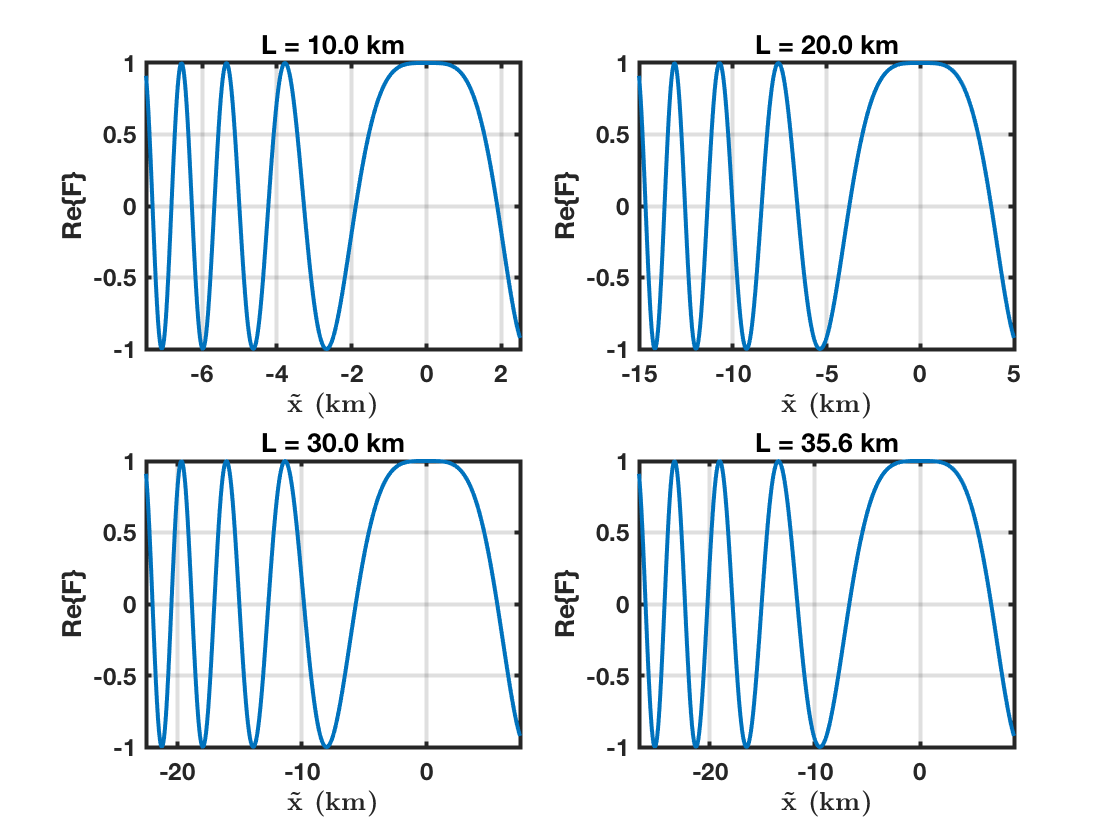
\includegraphics[width=4in]{../media/analysis/phaseVariation_30_10}
  \end{center}
  \renewcommand{\baselinestretch}{1} \small\normalsize
  \begin{quote}
    \caption[Real Part of Integrand for $h_1$ = 30m, $h_2$ = 10m]{ Real Part of Integrand for $h_1$ = 30m, $h_2$ = 10m\label{mp_fig:3}}
  \end{quote}
\end{figure}
\renewcommand{\baselinestretch}{2} \small\normalsize

\begin{figure}[H]
  \begin{center}
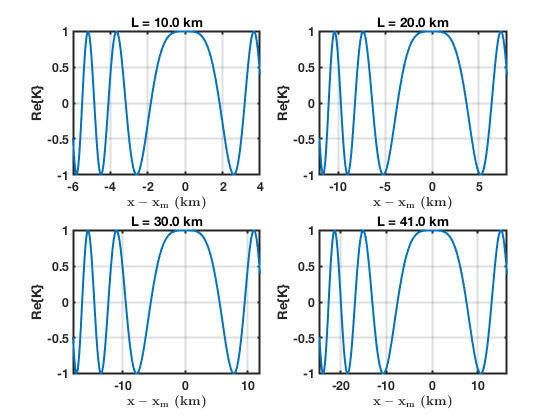
\includegraphics[width=4in]{../media/analysis/phaseVariation_30_20}
  \end{center}
  \renewcommand{\baselinestretch}{1} \small\normalsize
  \begin{quote}
  \caption[Real Part of Integrand for $h_1$ = 30m, $h_2$ = 20m]{ Real Part of Integrand for $h_1$ = 30m, $h_2$ = 20m\label{mp_fig:4}}
  \end{quote}
\end{figure}
\renewcommand{\baselinestretch}{2} \small\normalsize

\begin{figure}[H]
  \begin{center}
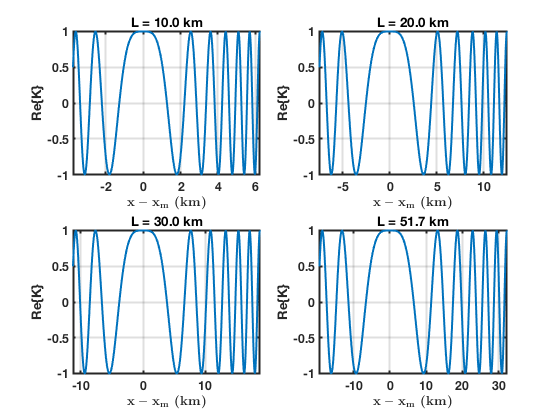
\includegraphics[width=4in]{../media/analysis/phaseVariation_30_50}
  \end{center}
  \renewcommand{\baselinestretch}{1} \small\normalsize
  \begin{quote}
  \caption[Real Part of Integrand for $h_1$ = 30m, $h_2$ = 50m]{ Real Part of Integrand for $h_1$ = 30m, $h_2$ = 10m\label{mp_fig:5}}
  \end{quote}
\end{figure}
\renewcommand{\baselinestretch}{2} \small\normalsize

Even with low altitudes, the phase oscillations will be rapid as $\tilde{x}$ goes past the limits of integration and will cancel out, so we can use the principle of stationary phase and let the positive limit extend to $\infty$. For each case shown, the carrier frequency of the electromagnetic wave was set to 35 GHz. Lower frequencies will have fewer oscillations, but the pricinple of stationary phase will still apply.

\begin{equation}
\begin{aligned}
I&=\int\limits_{0}^{\infty}dx\gamma(x)\exp\left[\frac{-jk_oL_0''}{2}(x-x_m)^2\right]\\
\end{aligned}
\label{mp_eq:23}
\end{equation}

To solve this equation, we can work in the complex plane as shown in Figure \ref{mp_fig:6}. The contour along the real axis, $\mathcal{C}_1$, is deformed to ensure we do not cross through the singular point at $\tilde{x} = L-x_m$ as given in Equation \ref{mp_eq:13} for the initial expression of $L_0$. From Jordan's Lemma, the contour along the arc $\mathcal{C}_2$ will be $0$. Since there are no singular points enclosed by the contour, the sum of the integrals along the contours is $0$ so that

\begin{equation}
I = -\int_{\mathcal{C}_3}d\tilde{x} \gamma(\tilde{x})\exp\left[\frac{-jk_oL_0''}{2}\tilde{x}^2\right]
\label{mp_eq:24}
\end{equation}

\begin{figure}[H]
  \begin{center}
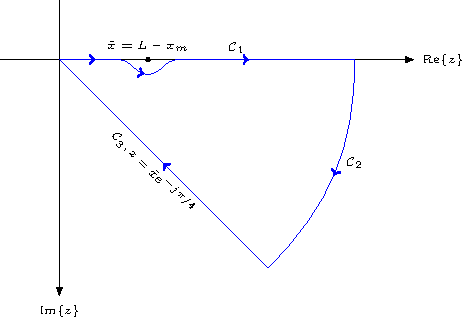
\includegraphics[width=5in]{../media/path_contour-figure1.pdf}
  \end{center}
  \renewcommand{\baselinestretch}{1} \small\normalsize
  \begin{quote}
    \caption[Path Contour]{ Path Contour\label{mp_fig:6}}
  \end{quote}
\end{figure}
\renewcommand{\baselinestretch}{2} \small\normalsize

To ensure we take the path of steepest descent, we can transform $\tilde{x}$ to the complex variable $z$ by applying a phase shift of $-\pi/4$, $\tilde{x} = z\exp[-j\pi/4]$. Now we can approximate the integral as

\begin{equation}
\begin{gathered}
I = -\int_{\mathcal{C}_3}d\tilde{z}e^{-j\pi/4} \gamma(\tilde{x})\exp\left[\frac{-k_oL_0''}{2}\tilde{z}^2\right]  \\
= e^{-j\pi/4}\int_{0}^{\infty}d\tilde{z}\gamma(\tilde{x})\exp\left[\frac{-k_oL_0''}{2}\tilde{z}^2\right]  \\
= e^{-j\pi/4}\gamma(x_m)\sqrt{\frac{2\pi}{k_oL_o''}} \\
\end{gathered}
\label{mp_eq:25}
\end{equation}

This yields an asymptotic approximation for the deterministic component of the integral as
\begin{equation}
\begin{gathered}
I = e^{-j\left(k_oL_{so}+\pi/4\right)}\Gamma_1 \sqrt{\frac{k_o}{2\pi jx_m}}\sqrt{\frac{k_o}{2\pi j (L-x_m)}}\frac{h_2}{L-x_m}\sqrt{\frac{2\pi}{k_oL_o''}} 
\end{gathered}
\label{mp_eq:26}
\end{equation}

We can simplify this expression by substituting in for $x_m$ and $L_0''$
\begin{equation}
\begin{gathered}
I= \Gamma_1e^{-j\left(k_oL_{so}+\pi/4\right)}\sqrt{\frac{k_o}{2\pi j\frac{h_1L}{h_1+h_2}}}\sqrt{\frac{k_o}{2\pi j (L-\frac{h_1L}{h_1+h_2})}}\frac{h_2}{L-\frac{h_1L}{h_1+h_2}}\sqrt{\frac{2\pi}{k_o\frac{(h_1+h_2)^4}{h_1h_2L^3}}} \\
= \Gamma_1e^{-j\left(k_oL_{so}+\pi/4\right)} \sqrt{\frac{k_o(h_1+h_2)}{2\pi jh_1L}}\sqrt{\frac{k_o(h_1+h_2)}{2\pi jLh_2}}\frac{h_2(h_1+h_2)}{Lh_2}\sqrt{\frac{2\pi h_1h_2L^3}{k_o(h_1+h_2)^4}} \\
= \Gamma_1e^{-j\left(k_oL_{so}+\pi/4\right)}  \sqrt{\frac{h_1+h_2}{h_1}}\sqrt{\frac{k_o}{2\pi j L}}\sqrt{\frac{h_1+h_2}{h_2}}\frac{h_1+h_2}{L}\sqrt{\frac{2\pi h_1h_2L^3}{k_o(h_1+h_2)^4}}\frac{1}{\sqrt{j}} \\
= \Gamma_1e^{-j\left(k_oL_{so}+\pi/4\right)}\sqrt{\frac{k_o}{2\pi jL}}e^{-j\pi/4} \\
= \Gamma_1e^{-j\left(k_oL_{so}+\pi/2\right)}\sqrt{\frac{k_o}{2\pi jL}} \\
\end{gathered}
\label{mp_eq:27}
\end{equation}

The asymptotic solution for the reflected wave in the paraxial assumption is then
\begin{equation}
\begin{gathered}
U_2(P-2)= \frac{1}{2jk_o}\sqrt{\frac{k_0}{2\pi jL}} \Gamma_1e^{-j\left(k_oL_{so}+\pi/2\right)} \\]
\label{mp_eq:27a}
\end{gathered}
\end{equation}
\renewcommand{\baselinestretch}{2} \small\normalsize

\section{Propagation Factor}
The propagation factor is then the sum of the two solutions and will include all the reflected paths from the surface

The full propagation factor is then given as
\begin{equation}
\begin{gathered}
F_p= \frac{1}{2jk_o}\sqrt{\frac{k_0}{2\pi jL}}\left[e^{-jkL_1} + \Gamma_1e^{-j\left(k_oL_{so}+\pi/2\right)}\right] \\
\end{gathered}
\label{mp_eq:27b}
\end{equation}

And can be normalized to the final result
\begin{equation}
\begin{gathered}
\boxed{F_p= e^{-jkL_1} + \Gamma_1e^{-j\left(k_oL_{so}+\pi/2\right)}} \\
\end{gathered}
\label{mp_eq:28}
\end{equation}

The asymptotic solution to the normalized propagation factor is the same expression as the 2 ray model but with an added phase shift.